\documentclass[xcolor=dvipsnames]{beamer}
\usepackage[utf8]{inputenc}
\usepackage{xcolor}
\usepackage{graphicx}
\usepackage{MnSymbol}
\usepackage{stmaryrd}
\usepackage{colortbl}
\usepackage{caption}
\usepackage{comment}
\usepackage[utf8]{inputenc}
\usepackage{pdfpages}
\usepackage{listings}
\usepackage{color}
\usepackage{booktabs}
\usepackage{soul}
\usepackage[normalem]{ulem}


\usepackage{tcolorbox}
\usepackage{lipsum}


%%%%%%%%%%%%%%%%%%%%%%%%%%%%%%%%%%%%%%%%%%%%%%%%%

\usepackage{pgf}
\usepackage{etex}
\usepackage{tikz,pgfplots}


\usetheme{Antibes}
%\usetheme{Madrid}
%\usecolortheme[named=Maroon]{structure}
\usecolortheme{dolphin}
\usefonttheme{professionalfonts}
\useoutertheme{infolines}
\useinnertheme{circles}

\newtheorem*{bem}{Bemerkung}

\usepackage{tikz}


%%%%%%%%%%%%%%%%%%%%%%%%%%%%%%%%%%%%%%%%%%%%%%%%%



%%%%%%%%%%%%%%%%%%%%%%%%%%%%%%%%%%%%%%%%%%%%%%%%%
\usepackage{listings}
\usepackage{color}

\definecolor{dkgreen}{rgb}{0,0.6,0}
\definecolor{gray}{rgb}{0.5,0.5,0.5}
\definecolor{mauve}{rgb}{0.58,0,0.82}

\lstset{frame=tb,
  language=Java,
  aboveskip=2mm,
  belowskip=2mm,
  showstringspaces=false,
  columns=flexible,
  basicstyle={\small\ttfamily},
  numbers=none,
  numberstyle=\tiny\color{gray},
  keywordstyle=\color{blue},
  commentstyle=\color{dkgreen},
  stringstyle=\color{mauve},
  breaklines=true,
  breakatwhitespace=true,
  tabsize=2
}
%%%%%%%%%%%%%%%%%%%%%%%%%%%%%%%%%%%%%%%%%%%%%%%%%


\title{Broj $e$ i primena u finansijama}
\author[Jovanović, Milenković, Milenković, Divjak]{Nikola Jovanović \\ Nikolina Milenković \\  Kristina Milenković \\ Anastasija Divjak}
\institute{Univerzitet u Beogradu, Matematički fakultet}
\logo{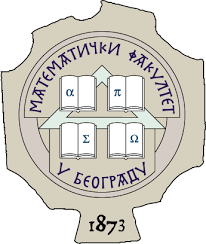
\includegraphics[height=2cm]{logo matf.png}}
\date{Beograd, Decembar 2022.}


\begin{document}

\begin{frame}
  \titlepage
\end{frame}

\begin{frame}
\frametitle{Rezime}
\begin{itemize}
 \item Otkriven 1618., nije mu pridavan veliki značaj
 \item Znatno kasnije švajcarski naučnik Leonard Ojler
 \item $e$ = 2,71828..., osnova prirodnog logaritma
 \item Prvobitni problem vezan za broj $e$ - finansije
\end{itemize}
\end{frame}

\section{Uvod}
\begin{frame}{Uvod}
\begin{block}{Istorija broja $e$}
    \begin{itemize}
        \item Prvo pojavljivanje - 1618. god (logaritamske tablice)
        \item 17. vek - Danijel Bernuli, ispitivanje u okviru bankarstva
        \item Pedesetak godina kasnije broj e napokon izračunat
    \end{itemize}
\end{block}
\end{frame}
\begin{frame}
\begin{block}{O Leonardu Ojleru}
    \begin{itemize}
        \item Rodjen u Bazelu 15. aprila 1707. godine
        \item Najveći doprinos u matematičkoj notaciji
        \item Pokušaj formulisanja teorije muzike zasnovane na matematici
    \end{itemize}
\end{block}
\vspace{5mm}
 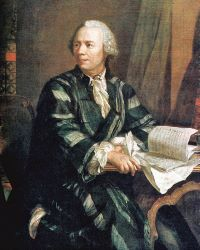
\includegraphics[height = 4cm, width = 3cm]{lojlermodified.jpg}
  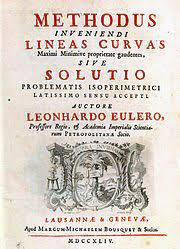
\includegraphics[height = 4cm, width = 3cm]{delo.png}
  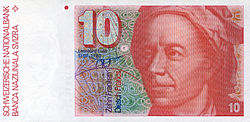
\includegraphics[height = 3cm, width = 4cm] {image.jpg}

\end{frame}
\section{Osobine broja $e$}
\begin{frame}
\begin{block}{Osobine broja $e$}
    \begin{itemize}
        \item iracionalan;
        \item realan;
        \item transcedentan;
        \item koristiti se u različitim granama matematike;
        \item predstavlja prirodan rast;
    \end{itemize}
    \begin{center}

		\begin{tabular}{|c|c|c|c|c|c|c|c|c|}
			\hline 
			n & 0 & 1 & 2 & 3 & 4 & 5 & 6 & 100 \\
			\hline
			$( 1 + \frac{1}{n} )^n$ & - & 2 & 2,25 & 2,3704 & 2,4414 & 2,4883 & 2,5216 & 2,7048 \\
			\hline
   
		\end{tabular}
	\end{center}
\end{block}   
\end{frame}

\section{Osobine broja $e$}
\begin{frame}
\begin{block}{Osobine broja $e$}
    \begin{itemize}
        \item predstavlja graničnu vrednost limesa: $\lim_{n\to\infty} ( \, 1 + \frac{1}{n} 	) \,^n$
        $\lim_{n\to\infty} ( \, 1 + \frac{1}{n} 	) \,^n =\lim_{n\to\infty} ( \, 1 + \frac{1}{3n} ) \,^\frac{3n}{3}= (\lim_{n\to\infty} ( \, 1 + \frac{1}{3n} ) \,^3n)^\frac{1}{3}= e^\frac{1}{3}$

	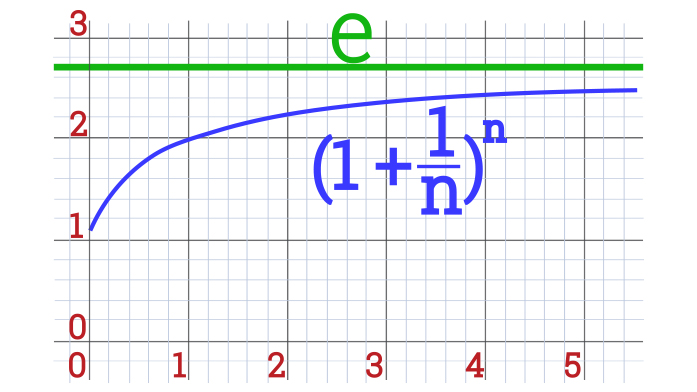
\includegraphics[height = 2.5cm, width = 4cm]{grafikon.jpg}
    \end{itemize}
    \begin{itemize}
        \item predstavlja sumu beskonačnog niza: \[ e= \sum_{n=0}^{\infty} \frac{1}{n!} = \frac{1}{0!} + \frac{1}{1!} + \frac{1}{2!} + \frac{1}{3!} + ... \]
        zbir prvih šest članova ovog niza iznosiće: \[ 1 + 1 + \frac{1}{2} + \frac{1}{6} + \frac{1}{24} + \frac{1}{120} = 2,718055556 \]
    \end{itemize}
\end{block}
\end{frame}
\section{Ojlerov identitet}
\begin{frame}
\begin{block}{Ojlerov identitet}
    \begin{itemize}
        \item Ojlerov identitet je naziv za formulu:$e^{i\phi}=\cos\phi+\sin\phi$;
        \item Važi za $\phi\in\mathbb{C}$;
        \item Za $\phi=\pi \ => \ e^{i\pi}=-1 \ => \ e^{i\pi}+1=0$;
        \item Fundamentalni brojevi $i, \pi, e, 1$, i $0$;
    \end{itemize}
\end{block}
    \begin{center}
    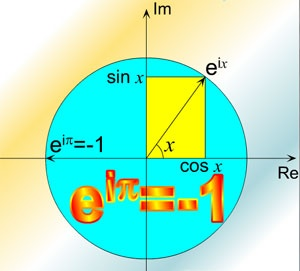
\includegraphics[height = 4cm]{ojlerova_kruznica1.jpg}
    \end{center}
\end{frame}

\section{Ojlerova kružnica}
\begin{frame}
\begin{block}{Ojlerova kružnica}
    \begin{itemize}
        \item Drugi naziv za Ojlrovu kružnicu je kružnica devet tačaka;
        \item Može se konstruisati za svaki trougao;
        \item Sadrži: podnožja visina trougla, podnožja težišnih duži trougla i sredine rastojanja ortocentra trougla od svakog temena;
    \end{itemize}
\end{block}
    \begin{center}
    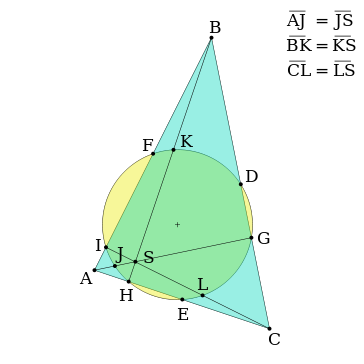
\includegraphics[height = 5cm]{ojlerova_kruznica2.png}
    \end{center}
\end{frame}

     \section{O Bernuliju}
    \begin{frame}
    \begin{block}{O Bernuliju}
    \begin{itemize}
        \item Sticao je znanja iz matematike i
          prirodnih nauka, takodje je bio i predavač\\
        \item Bio je prijatelj Leonarda Ojlera\\
        \item Bavio se raznim matematičkim problemima\\
    \end{itemize}
   \end{block}
    \begin{center}
    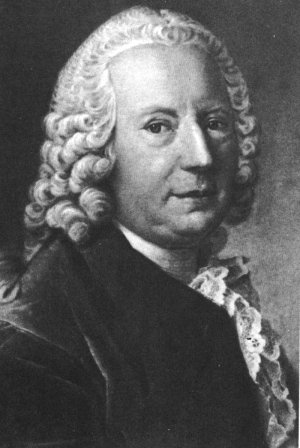
\includegraphics[height=4.cm]{bernuli.jpg}
    \end{center}
  \end{frame}
        
       \section{Primena u finansijama i zaključak}
    \begin{frame}
    \begin{block}{Primena u finansijama i zaključak}
     Pretpostavimo da u banku ulažemo sumu novca x:\\
    \begin{itemize}
        \item 100 posto kamata -- dobijamo $2*x$ sumu novca \\
        \item  Sledi sledeća formula $( 1 + \frac{1}{2} )^2 * x$ , za godinu dana bi bilo  $( 1 + \frac{1}{365} )^{365} * x$ \\\\
    \end{itemize}
       \begin{equation}\lim_{n \rightarrow \infty} (1+\frac{1}{n})^n=e \end{equation}
   \end{block}
    \begin{center}
    
\includegraphics[height=3.cm]{SlikaE.png}
    \end{center}
   \end{frame}    
%%%%%%%%%%%%%%%%%%%%%%%%%%%%%%%%%%%%%%%%%%%%%%%%%%%
\end{document}
